\chapter{Vorgehen}
\label{ch:development_approach}

\section{Projektplanung}
\label{sec:project_plan}
Zur Realisierung einer forensischen Analyseplattform wurde ein Projektplan erstellt, welcher die einzelnen Aufgaben im Rahmen der Masterthesis enthält. Abbildung \ref{fig:workpackages} zeigt die Aufteilung in diese Arbeitspakete.\\
Das Ziel der Einarbeitungsphase ist, ein grundlegendes Verständnis über die Datenverarbeitung im Hadoop-Framework zu erhalten. Zusätzlich soll eine Entwicklungsumgebung inklusive öffentlicher Versionsverwaltung eingerichtet werden. Danach erfolgt der Aufbau eines eigenen Hadoop-Clusters und die Beschaffung von Testdaten.\footnote{Hierbei wird ein bestehendes Hadoop-Cluster genutzt und um zusätzliche Softwarepakete ergänzt.} Für die Einarbeitung und den Aufbau sind vier Wochen eingeplant (siehe Abbildung \ref{fig:ganttA}).\footnote{Die referenzierten Gantt-Diagramme wurden mit der JavaScript-Bibliothek \textit{dhtmlxGantt} erstellt. Der Quellcode ist unter der \textit{GNU GPLv2}-Lizenz lizenziert. Weiter Informationen können in Kapitel \ref{sec:licencing_issues} im Anhang nachgelesen werden.}\\

\noindent
Der zweite Teil behandelt die Datenaufbereitung und Speicherung im Hadoop-Cluster. Es soll geprüft werden, welche Struktur der Daten für eine optimale Speicherung und Verarbeitung im Hadoop-Framework erforderlich ist. Für diesen Teil sind vier Wochen Bearbeitungszeit geplant.\\
Am Ende des Arbeitspakets soll ein erster Zwischenbericht erstellt werden, welcher die bisherigen Ergebnisse enthält (sieh Abbildung \ref{fig:ganttA}).\\

\begin{figure}[ht]
  \centering
  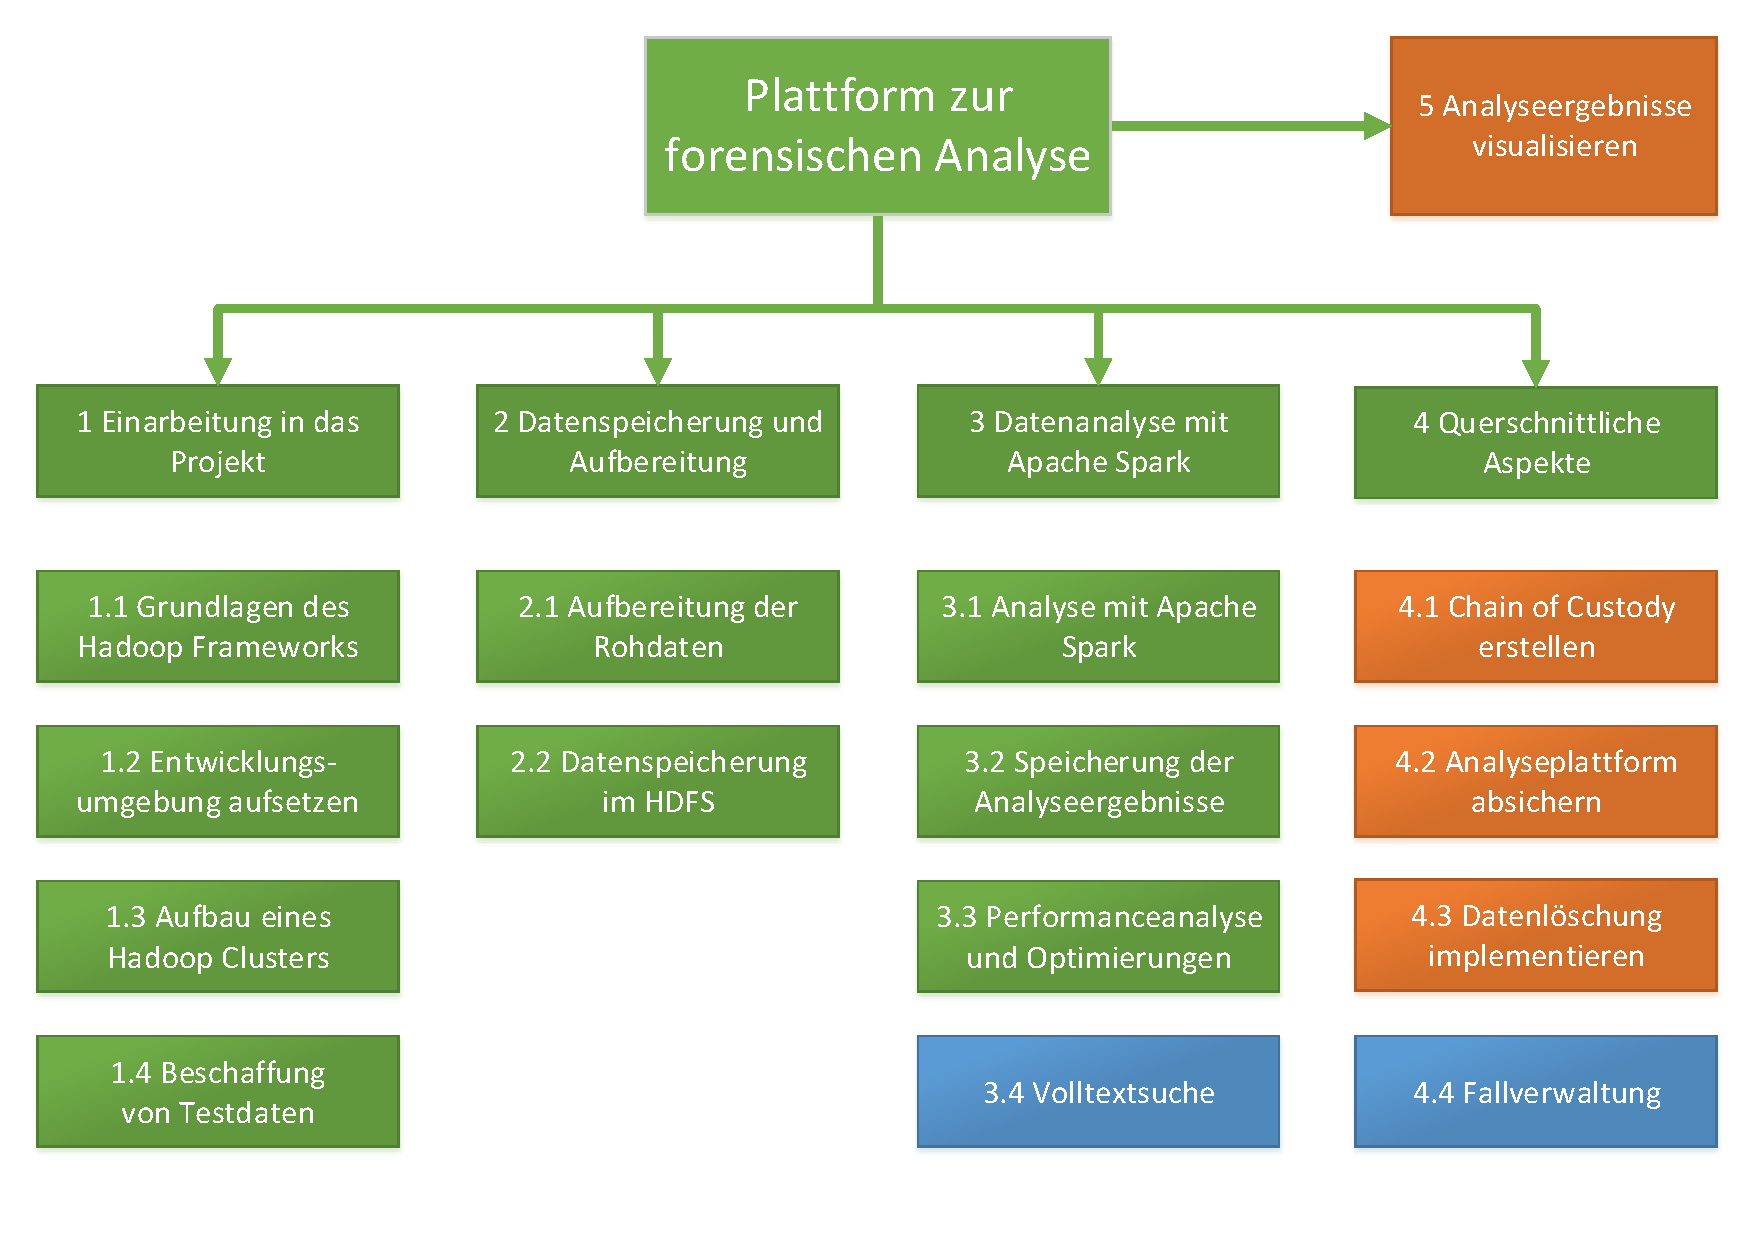
\includegraphics[width=\textwidth]{./resource/Arbeitspakete.pdf}
  \caption{Arbeitspakete der Masterthesis}
  \label{fig:workpackages}
\end{figure}

\noindent
Nach der Speicherung der Rohdaten erfolgt im dritten Arbeitspaket die Datenanalyse mit Apache Spark. Hier sollen die Daten nach anwendungsbezogenen Problemstellungen analysiert werden. Ein weiterer Aspekt der Datenanalyse beschäftigt sich mit den Möglichkeiten, wie die Ergebnisse persistiert werden können.\footnote{Dafür soll Apache HBase zur Speicherung von strukturierten und unstrukturierten Daten untersucht werden.}Im Anschluss soll die Performanz der Algorithmen geprüft werden. Hier bietet sich der Vergleich zu herkömmlichen Analyseprogrammen an. Denn schließlich hat diese Thesis auch das Ziel, bei großen Datenmengen schneller Ergebnisse zu liefern als die herkömmlichen Analysewerkzeuge auf einem einzelnen Analyserechner. Für dieses Arbeitspaket sind sieben Wochen eingeplant (siehe Abbildung \ref{fig:ganttB}).\\
 Darauf folgt ein zweiter Zwischenbericht.\\

\noindent
Im letzten Drittel der Masterthesis sollen querschnittliche Aspekte in die bestehende Analyseplattform integriert werden. Hierbei geht es um das Absichern der Plattform, die Dokumentation der Beweismittelkette und um das sichere Löschen von Asservaten. Für dieses Arbeitspaket sind vier Wochen eingeplant (siehe Abbildung \ref{fig:ganttC}).\\

\noindent
Das letzte Arbeitspaket enthält ein prototypische Visualisierung der Analyseergebnisse. Hierbei soll geprüft werden, welche Möglichkeiten zur Darstellung der Ergebnisse existieren. Für diese Arbeit sind drei Wochen eingeplant (siehe Abbildung \ref{fig:ganttC}).\\

\subsection*{Projektverlauf}
Während dem Projektverlauf wurde die Planung teilweise angepasst. Es wurden einige Aspekte aus der Planung entfernt (orange hinterlegt in Abbildung \ref{fig:workpackages}). So wurden die Visualisierung der Ergebnisse, die Erstellung der Beweismittelkette, das Absichern der Analyseplattform und die forensisch korrekte Datenlöschung nicht implementiert sondern nur theoretisch erläutert. Der Hauptgrund dafür, war eine intensive Analyse und Entwicklung, wie die Daten im Hadoop-Cluster gespeichert werden können. Hier wurden mehrere Varianten getestet und die ursprünglich angedachte Bearbeitungszeit verlängerte sich.\\

\noindent
Andererseits sind auch neue Arbeitspakete hinzugekommen (blau hinterlegt in Abbildung \ref{fig:workpackages}). So wurde bei der Datenanalyse mit Apache Spark sichtbar, dass die Informationen und Analyseergebnisse performant durchsuchbar sein müssen. Daher wurde untersucht, wie eine Volltextsuche aller gespeicherten Daten im Hadoop-Cluster realisiert werden könnte.\\
Ein anderer Aspekt ist die Implementierung einer Fallverwaltung. Denn damit können nun mehrere Asservate in das System importiert werden, um Zusammenhänge identifizieren zu können. 

\begin{figure}[p]
  \centering
  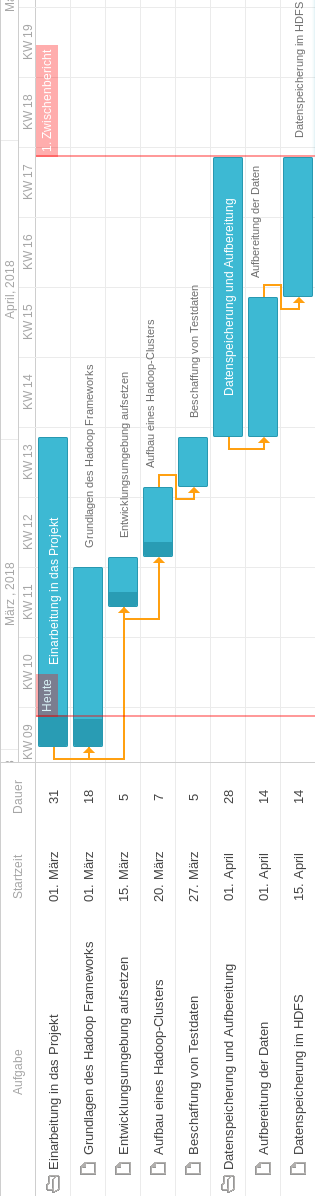
\includegraphics[width=\textwidth,height=\textheight,keepaspectratio]{./resource/ganttA.png}
  \caption{Projektplan Teil A - Einarbeitung und Rohdatenspeicherung (siehe Kapitel \ref{sec:licencing_issues})}
  \label{fig:ganttA}
\end{figure}

\begin{figure}[p]
  \centering
  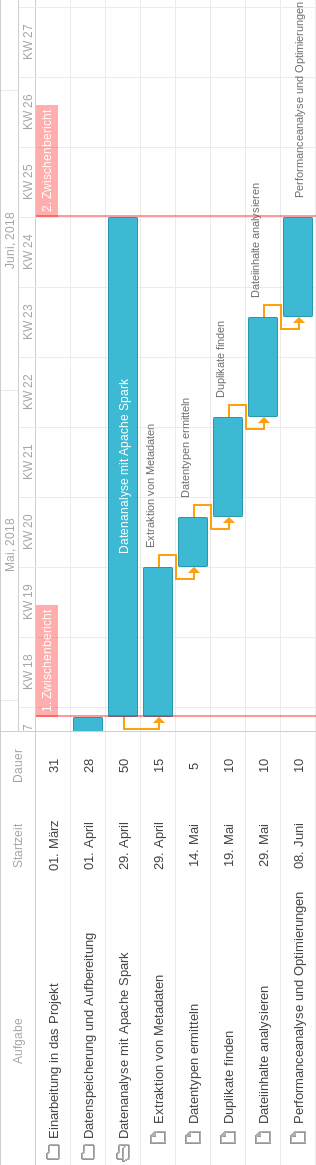
\includegraphics[width=\textwidth,height=\textheight,keepaspectratio]{./resource/ganttB.png}
  \caption{Projektplan Teil B - Datenanalyse (siehe Kapitel \ref{sec:licencing_issues})}
  \label{fig:ganttB}
\end{figure}

\begin{figure}[p]
  \centering
  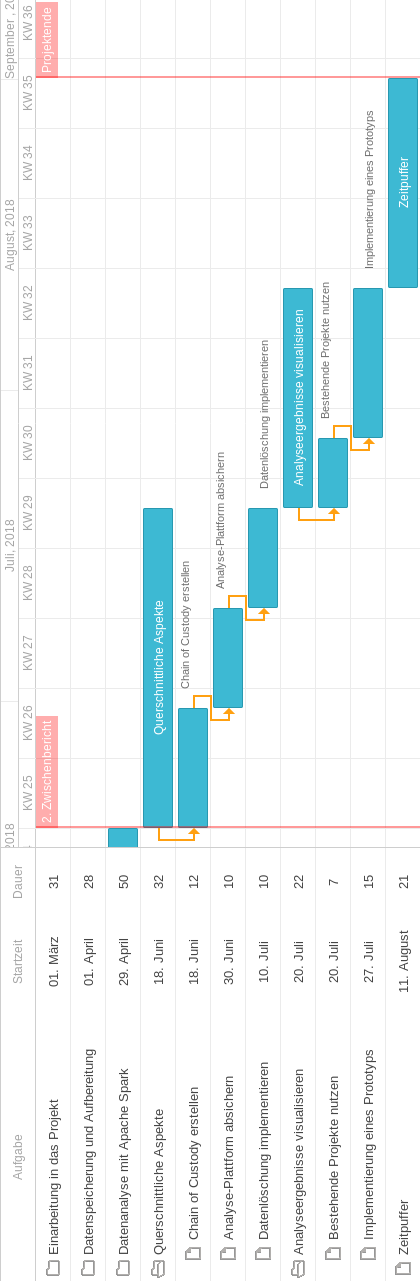
\includegraphics[width=\textwidth,height=\textheight,keepaspectratio]{./resource/ganttC.png}
  \caption{Projektplan Teil C - Querschnittliche Aspekte und Visualisierung (siehe Kapitel \ref{sec:licencing_issues})}
  \label{fig:ganttC}
\end{figure}

\clearpage
\section{Entwicklungsumgebung}
\label{development_environment}
Der Aufbau eine Test- und Entwicklungsumgebung ist ein wichtiger Bestandteil dieser Thesis. Einerseits sollen Anwendungsprogramme zur Datenverarbeitung schnell und lokal ausführbar sein. Andererseits soll die Testumgebung auf einem physikalischem Apache Hadoop Cluster basieren, um mögliche Infrastrukturprobleme identifizieren zu können und die Performanz zu testen. \\

\noindent
Abbildung \ref{fig:development_environment} skizziert die Komponenten der Entwicklungsumgebung. Zentraler Bestandteil ist ein Entwicklungsrechner mit der Linux-Distribution \textit{Fedora} in der Version 28 64-bit.

\begin{figure}[ht]
  \centering
  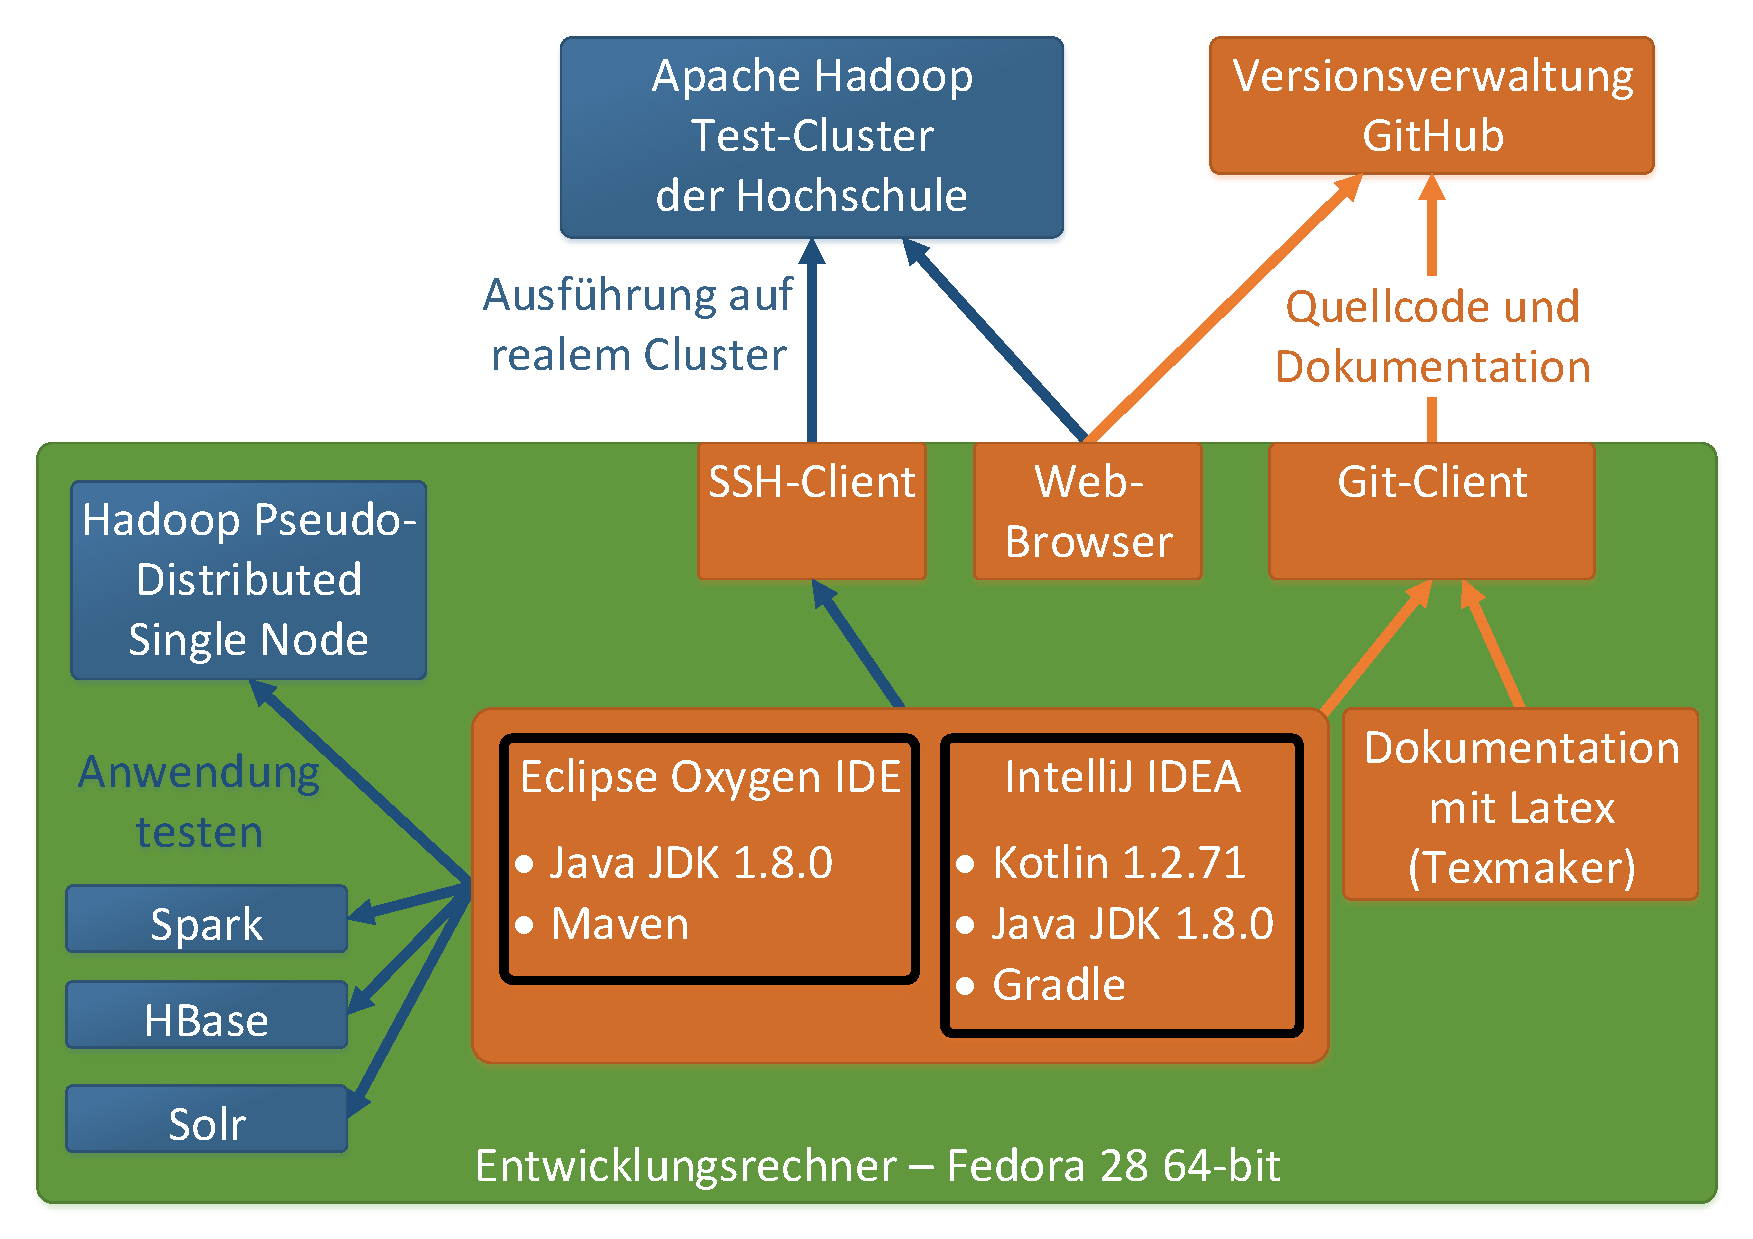
\includegraphics[width=\textwidth]{./resource/development_environment.pdf}
  \caption{Komponenten der Entwicklungsumgebung}
  \label{fig:development_environment}
\end{figure} 

\noindent
Zur Entwicklung der forensischen Analyseprogramme wird \textit{Eclipse Oxygen} genutzt. Die Anwendungen selbst werden in Java geschrieben.\footnote{Wobei auch Python oder Scala als Programmiersprache genutzt werden kann.} Zum Bauen der ausführbaren \gls{jar} wird \textit{Maven} verwendet. Mit Maven können weitere Java-Bibliotheken 
in eigenen Programmen auf einfache Weise wiederverwendet werden.\footnote{Diese können über ein zentrales Repository, dem sogenannten \textit{Maven Central Repository} aus dem Internet geladen werden (siehe Link\url{https://search.maven.org/}. Letzter Zugriff 26.8.2018).}\\

\noindent
Zusätzlich befindet sich die Entwicklungsumgebung \textit{IntelliJ IDEA} in der kostenlosen Cummunity Variante  auf dem Entwicklungsrechner. Mit der IntelliJ IDEA wird die Datenimport-Anwendung in \textit{Kotlin} entwickelt. Kotlin ist eine statisch typisierte Programmiersprache zur Anwendungsentwicklung auf verschiedenen Plattformen.\footnote{Siehe Link \url{https://kotlinlang.org/}. Letzter Zugriff: 24.8.2018.} Sie ist interoperabel mit Java. Die Anwendungen können in der \textit{Java Virtual Machine} (JVM) ausgeführt werden. Gegenüber Java bietet sie diverse Sprachkonstrukte zur Optimierung des Programmcodes an. Darüber hinaus können alle Bibliotheken aus dem Java-Umfeld auch in Kotlin genutzt werden. Zum Bauen der Kotlin-Anwendungen wird \textit{Gradle} genutzt, welches analog zu Maven Abhängigkeiten zu Drittbibliotheken und deren Versionen verwaltet.\footnote{Siehe auch Kapitel \ref{subsec:data_import_implementation} für weitere Informationen zur Datenimportanwendung.}\\


\noindent
Um die gebauten Java- und Kotlin-Programme schnell zu testen, können alle notwendigen Komponenten auch lokal auf dem Entwicklungsrechner gestartet werden. Hierzu gehört ein Hadoop-Knoten im sogenannten \textit{Pseudo-Distributed} Modus, eine lokale Spark-Instanz, eine HBASE-Instanz und eine Solr-Instanz zur Datenindexierung.\footnote{Siehe Kapitel \ref{ch:theory_hadoop} für eine detaillierte Erklärung der Komponenten.}\\
Mithilfe dieser Komponenten können auch spezifische Konfigurationen getestet werden.\footnote{Hierfür muss der Entwicklungsrechner entsprechende Ressourcen bereitstellen. Es sollte mindestens eine Quad-Core-CPU, 16 GB Arbeitsspeicher und eine SSD zur Verfügung stehen, um performant arbeiten zu können.} \\
Letztendlich kommen die lokalen Instanzen schnell an ihre Grenzen, gerade wenn größere Datenmengen analysiert werden sollen. Daher werden spezifische Konfigurationen und fertiggestellte Analyseprogramme auch auf einem realen
Apache Hadoop-Cluster durchgeführt. Dort kann das Zusammenspiel zwischen den Komponenten nachvollzogen werden. Auch entsprechende Last-Tests sind nur auf dem Hadoop Test-Cluster möglich. Um mit dem Test-Cluster arbeiten zu können, wird ein SSH-Client benötigt. Zusätzliche gibt es auch eine Web-Oberfläche basierend auf Apache Ambari zur Konfiguration und Anzeige des aktuellen Systemzustandes.\\

\noindent
Alle selbst erstellten Anwendungsprogramme, Konfigurationsdateien und die Dokumentation dieser Thesis sollen als Open-Source Projekte in einem öffentlichen Repository zugänglich sein. Aus fachlicher Sicht ist es gerade in der Forensik sehr wichtig dem Nutzer die Möglichkeit zu geben, den Quellcode der Analyseprogramme einsehen zu können und notfalls auf spezielle Bedürfnisse anzupassen. Darüber hinaus kann die Datenverarbeitung transparent nachvollzogen werden.
Daher werden die einzelne Projekte mithilfe eines Git-Clients auf GitHub versioniert.\\
Nachfolgende Auflistung zeigt die Aufteilung der Projekte:
\begin{itemize}
\item Das Projekt \textit{foam-thesis}\footnote{Die Abkürzung \textit{foam} oder auch \textit{foAm} steht für \textit{\textbf{fo}rensische \textbf{A}nalyseplattfor\textbf{m}}} enthält die schriftliche Ausarbeitung der Thesis und den Quellcode als Latex-Projekt. Als Entwicklungsumgebung wird \textit{Texmaker} genutzt.\\
Über den Link \url{https://github.com/jobusam/foam-thesis} ist der aktuelle Stand der Arbeit jederzeit einsehbar.\footnote{Das kompilierte PDF-Dokument zum jeweiligen Stand wird im gleichen Projekt versioniert und ist unter dem Link \url{https://github.com/jobusam/foam-thesis/blob/master/main.pdf} verfügbar.}

\item Das Projekt \textit{foam-data-import} enthält den Quellcode zum Importieren von Asservaten in das Hadoop-Cluster. Unter \url{https://github.com/jobusam/foam-data-import} befindet sich die Kotlin-Anwendung, welche wiederum mit Gradle gebaut werden kann.

\item Das Projekt \textit{foam-processing-spark} enthält den Quellcode zur Auswertung mit Apache Spark\texttrademark\thinspace. Unter \url{https://github.com/jobusam/foam-processing-spark} befindet sich ein Maven-Projekt, welches wiederum die Java-Anwendung baut. Es werden auch entsprechende Skripte zum Starten von Spark-Anwendungen auf dem lokalen Rechner bereitgestellt. 

%TODO Installationsskripte zu HBASE und Solr!
\item Das Projekt \textit{foam-storage-hadoop} enthält alle Konfigurationsdateien zum Aufsetzen eines Hadoop-Clusters auf einem einzelnem Knoten im \textit{Pseudo-Distributed Mode}.\footnote{Siehe Link \url{https://github.com/jobusam/foam-storage-hadoop/tree/master/hadoop.standalone.configuration}} Zusätzlich existieren Shell-Skripte zum Starten des Hadoop-Clusters auf einem einzelnen Knoten.\footnote{Siehe Link \url{https://github.com/jobusam/foam-storage-hadoop/tree/master/hadoop.standalone.setup}} Mithilfe der Skripte aus dem \textit{foam-processing-spark} Projekt können damit Spark-Anwendungen ausgeführt werden.
\end{itemize}

\noindent
Derzeit ist die Lizenzierung der Projekte noch unklar. Sehr wahrscheinlich wird die Thesis-Dokumentation unter der \textit{GNU Free Documentation License (GFDL)} lizenziert, wohingegen der restliche Quellcode unter der \textit{GNU Affero General Public License Version 3 (AGPLv3)} oder alternativ unter der Apache License 2.0 veröffentlicht werden soll. Es soll jedem möglich sein, den Quellcode einzusehen und nach belieben ändern zu können.\\

\section{Testdatengenerierung}
\label{testdatacreation}
\textbf{TODO: Kapitel durchlesen...}\\
Für den Aufbau einer forensischen Analyseplattform sollen entsprechende Testdaten generiert werden. Hierbei gibt es zwei unterschiedliche Falldaten. Der erste Fall wäre ein kleines Image mit knapp 10 GB. Dieses Image könnte für lokale Tests genutzt werden. Darauf wurde ein Ubuntu 16.04 LTS installiert. Danach wurden einige Dateien heruntergeladen.\\

\noindent
Im zweiten Fall wird ein 480 GB großes Image erzeugt. Hierzu wird aktuelles Windows 10 installiert. Danach werden größere Datensätze von Bildern und Musik aus dem Internet geladen. Diese Datensätze werden lizenzfrei als Trainingsdaten zum maschinellen Lernen angeboten. Dieses große Datenträgerabbild wird in Kapitel \ref{sec:performance_analysis} für Leistungstests genutzt. Hierzu sollten sich einige sehr große aber auch viele kleine Dateien im Abbild befinden.\\ 
%\noindent
%Für lokale Tests und den Aufbau der Plattform bietet sich beispielsweise auch das Testscenario \textit{Data Leakage Case} an, welches auf der Website \textit{Computer Forensic Reference Data Sets} verfügbar ist.\footnote{Siehe \url{https://www.cfreds.nist.gov/data_leakage_case/data-leakage-case.html},\\ letzter Stand 28.3.2018.} \\
%Diese Images könnten auf verdächtige Querverweise untersucht werden.